\documentclass[a4paper, 11pt, titlepage]{article}
\usepackage{ucs}
\usepackage[german,ngerman]{babel}
\usepackage{fontenc}
\usepackage[pdftex]{graphicx}
\usepackage{xcolor}
\usepackage{listings}


\definecolor{dunkelblau}{RGB}{16, 55, 188}
\definecolor{orange}{RGB}{255, 60, 0}
\definecolor{gruen}{RGB}{18, 118, 34}
\definecolor{gelb}{RGB}{255, 200, 0}
\definecolor{lila}{RGB}{147, 18, 114}
\lstdefinestyle{sql}{
language=sql,
 literate=
    {'}{{\textquotesingle}}1, % ' wird als Apostroph ausgegeben
commentstyle=\color{gruen}, 
keywordstyle =\color{dunkelblau}, 
%Bis hier hin Farbgebung
frame=single, % Umrandung des Codes
rulecolor=\color{lightgray},
numbers=left, % Nummerierung hinzufügen (links)
numberstyle=\tiny, % Stil der Zeilennummern
stepnumber=1, % Schrittzahl für die Nummerierung
numbersep=5pt, % Abstand zwischen Nummerierung und Code
basicstyle=\sffamily, % Ändert die Schriftart des Codes
tabsize = 4, %Tab-Abstand
breaklines=true, %Zeilenumbruch
showstringspaces=false
}

\renewcommand*{\thesubsection}{\alph{subsection}.}

\begin{document}
\title{Datenbanken \\
Ausarbeitung \"Ubung 10}

\author{Jakob Schulz}

\date{\today}

\maketitle{\thispagestyle{plain}}

\section{Aufgabe}
\subsection{DDL Anweisungen}
\lstinputlisting[style = sql]{ddl.sql}
\subsection{"Uberpr"ufen, ob Tabellen mit Daten bef"ullt wurden:}
\begin{lstlisting}[style = sql]
Select count(*)
from embarked
\end{lstlisting}
\begin{lstlisting}[style = sql]
Select count(*)
from tickets
\end{lstlisting}
\begin{lstlisting}[style = sql]
Select count(*)
from titanic
\end{lstlisting}
\subsection{ER-Diagramm}
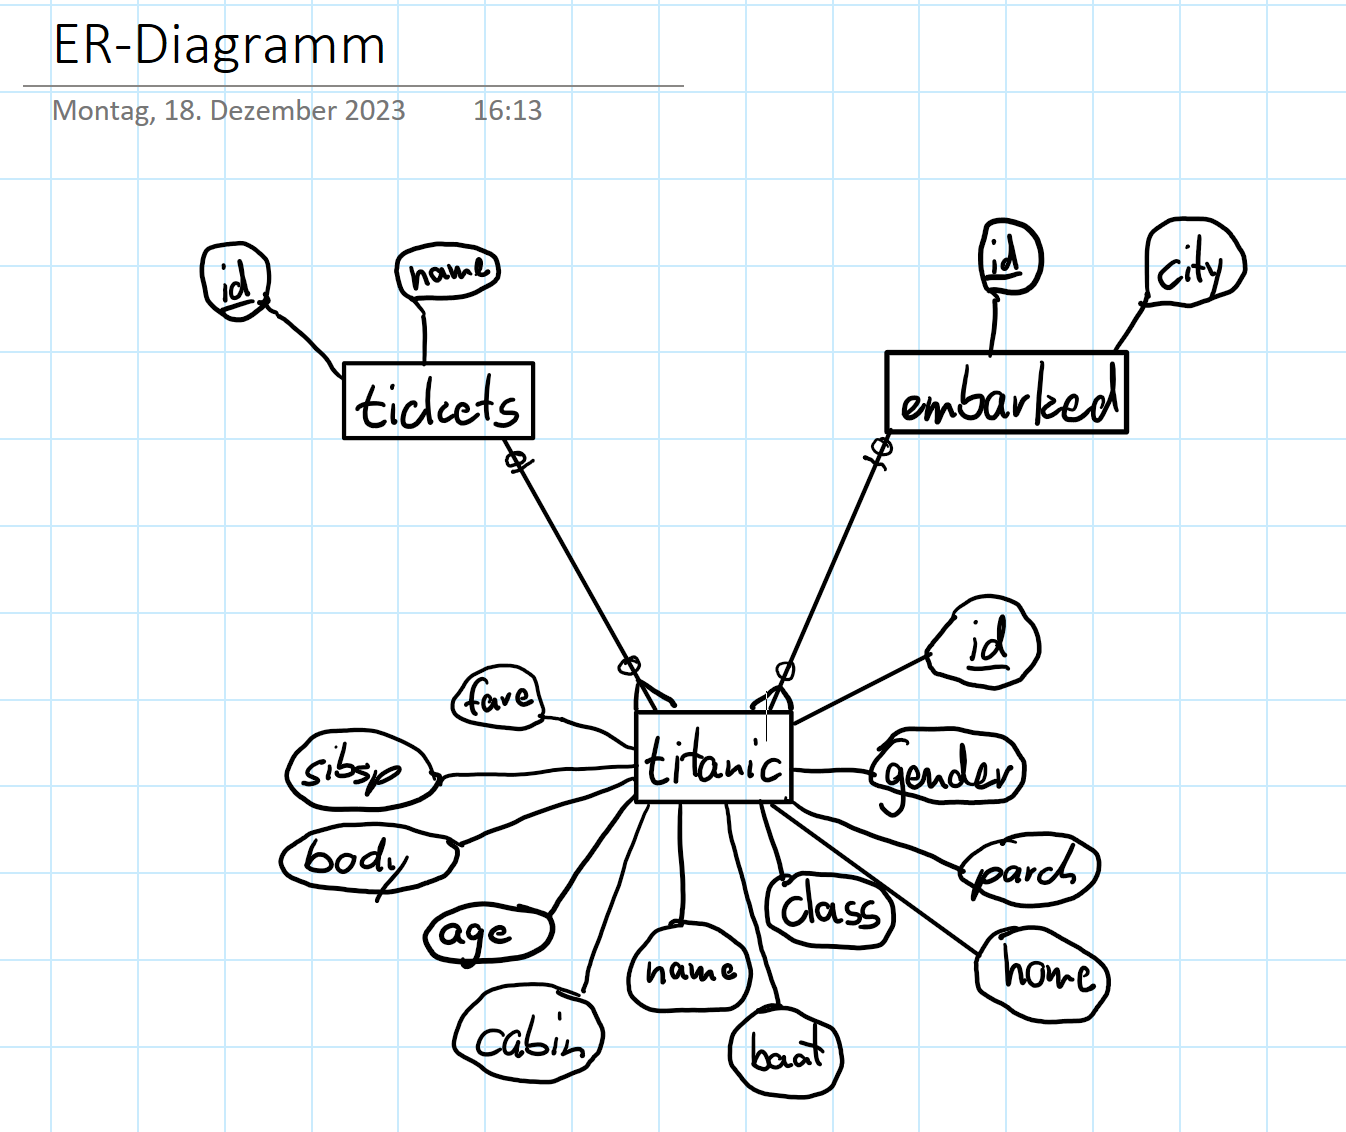
\includegraphics[width = 10cm]{ER-Diagramm.png}
\section{Aufgabe}
\subsection{Wie viele Passagiere sind in Southampton zugestiegen?}
\begin{lstlisting}[style = sql]
Select count(*)
from titanic, embarked
where titanic.embarked_id = embarked.id and embarked.city = 'Southampton'
\end{lstlisting}
\begin{lstlisting}[style = sql]
Select count(*)
from titanic 
inner join embarked on embarked.id = titanic.embarked_id
where embarked.city = 'Southampton'
\end{lstlisting}
\subsection{Von wie vielen Passagieren ist der Zustiegshafen unbekannt?}
\begin{lstlisting}[style = sql]
Select count(*)
from titanic
where embarked_id is null
\end{lstlisting}
\begin{lstlisting}[style = sql]
Select count(*)
from titanic left
outer join embarked on embarked.id = titanic.id
where embarked_id is null
\end{lstlisting}

\subsection{In welchem Hafen ist der Passagier namens Lovell zugestiegen?}
Welche Nummer hat sein Ticket?
\begin{lstlisting}[style = sql]
Select titanic.name as Name, embarked.city as Zustiegshafen, tickets.name as Ticketnummer
from titanic, tickets, embarked
where titanic.embarked_id = embarked.id and titanic.ticket_id = tickets.id and titanic.name like '%Lovell%';
\end{lstlisting}
\begin{lstlisting}[style = sql]
Select titanic.name as Name, embarked.city as Zustiegshafen, tickets.name as Ticketnummer
from titanic
inner join embarked on titanic.embarked_id = embarked.id
inner join tickets on titanic.ticket_id = tickets.id
where titanic.name like '%Lovell%';
\end{lstlisting}
\subsection{Wie viele Passagieren sind jeweils in den drei verschiedenen Häfen zugestiegen?}
\begin{lstlisting}[style = sql]
Select embarked.city, count(*)
from titanic, embarked
where embarked.id = titanic.embarked_id
group by embarked.city
\end{lstlisting}
\begin{lstlisting}[style = sql]
Select embarked.city, count(*)
from titanic 
inner join embarked on embarked.id = titanic.embarked_id
group by embarked.city
\end{lstlisting}
\verb+group by embarked.id+ funktioniert auch, aber laut seiner Vorlesung m"usste man group by embarked.city verwenden
\subsection{Gesucht sind Name, Ticketnummer aus der Spalte 'name' in der Tabelle 'tickets'
und der Zustiegshafen des Passagiers mit der ID 1014}
\begin{lstlisting}[style = sql]
Select titanic.name, tickets.name as Ticketnummer, embarked.city as Zustiegshafen
from titanic, tickets, embarked
where titanic.embarked_id = embarked.id and titanic.ticket_id = tickets.id and titanic.id = 1014
\end{lstlisting}
\begin{lstlisting}[style = sql]
Select titanic.name, tickets.name as Ticketnummer, embarked.city as Zustiegshafen
from titanic
inner join embarked on titanic.embarked_id = embarked.id 
inner join tickets on titanic.ticket_id = tickets.id
where titanic.id = 1014
\end{lstlisting}
\subsection{Welche Tickets wurden von mehreren Personen genutzt?}
Gesucht sind die Werte aus der Spalte 'name' in der Tabelle 'tickets'
\begin{lstlisting}[style = sql]
Select tickets.name
from tickets, titanic
where tickets.id = titanic.ticket_id
group by tickets.name
having count(*)  > 1
\end{lstlisting}
\begin{lstlisting}[style = sql]
Select tickets.name
from titanic
inner join tickets on tickets.id = titanic.ticket_id
group by tickets.name
having count(*)  > 1
\end{lstlisting}
\subsection{Gibt es Personen, die mit dem gleichen Ticket gereist sind, aber in verschieden Häfen 
zugestiegen sind?}
Gesucht sind die Namen, die Ticketnummer und die Zustiegshäfen.\\
Man kann auf Grund von group by nur die Ticketnummer ausgeben, aber nochmal nachfragen.
\begin{lstlisting}[style = sql]
Select tickets.name as Ticketnummer
from titanic, tickets
where tickets.id = titanic.ticket_id
group by tickets.name
having count(titanic.name) > 1 and count(distinct titanic.embarked_id) > 1
\end{lstlisting}
\begin{lstlisting}[style = sql]
Select tickets.name as Ticketnummer
from titanic
inner join tickets on tickets.id = titanic.ticket_id
group by tickets.name
having count(titanic.name) > 1 and count(distinct titanic.embarked_id) > 1
\end{lstlisting}
\end{document}